\documentclass{article}

\usepackage[english]{babel}
\usepackage[utf8]{inputenc}
\usepackage{kpfonts}
\usepackage[left=2.8cm, right=2.8cm, top=2.8cm, bottom=3cm]{geometry}
\usepackage{titling}
\usepackage{graphicx}
\usepackage{hyperref}
\usepackage{tikz}
\usepackage{amsmath}

\graphicspath{{ims/}}

%%%%%%%%%%%% Title Part %%%%%%%%%%%%
\pretitle{
	\begin{center}
	\includegraphics[width=4cm]{logo_ens_lyon.pdf}
	\hspace{5cm}
	
\includegraphics[width=5.5cm]{logo_tu_delft.png}
	\LARGE
}
\title{
	\rule{\linewidth}{0.4mm}
	\textbf{Perspective Check in Paintings} \\
	\textit{M1 Internship}
	\rule{\linewidth}{0.6mm}
}
\author{
	Yoann Coudert--Osmont \\[3mm]
	\textit{Supervised by} \\
	Elmar Eisemann \qquad Ricardo Marroqium \\[2mm]
}
\date{May - July 2019}
%%%%%%%%%%%%%%%%%%%%%%%%%%%%%%%%%%%%

\begin{document}
	\maketitle
	
	\section*{Introduction}
	
	\begin{figure}
		\centering
		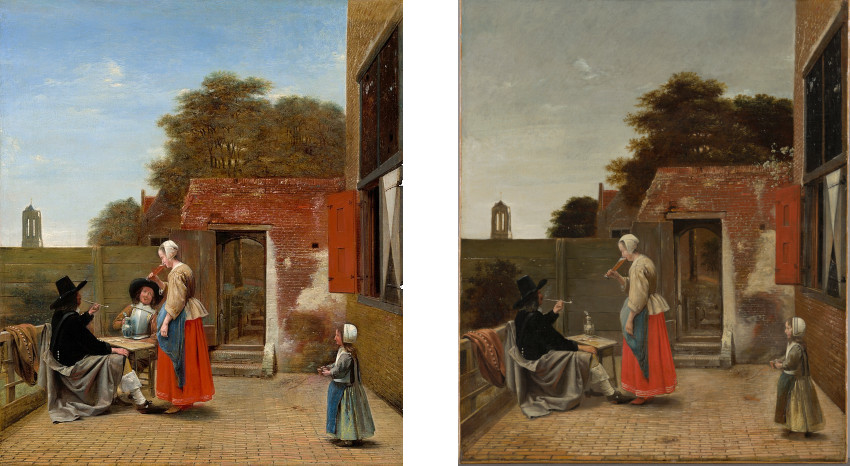
\includegraphics[scale=1.25]{paintings_pair.jpg}
		\caption{A pair of similar paintings}
		\label{im:pair}
	\end{figure}

	In a Delft museum, paintings by Pieter de Hooch are on display. It is quite easy to notice that some pairs of paintings are very similar (e.g. \figurename \ref{im:pair}). One hypothesis that would explain this strangeness is the possibility that another painter copied Pieter de Hooch's paintings. Looking at the pairs in more detail, we can notice that quite often one painting respects the rules of perspective well and the other does not respect them. This gives credibility to the hypothesis of the existence of another painter. But the human tends to be biased to check that in each pair one painting respects the rules of perspective and the other does not. Then comes the need to create a tool to check whether the perspective is respected in a painting with as little human intervention as possible. The goal of this internship was therefore to create a graphical interface to verify the perspective in a painting with as much automation as possible. \\
	Tools already exist to find lines in an image. The most common and the one I used is the Hough transform \cite{hough}. I will describe the algorithms used to create my interface in this report. The development of a graphical user interface with minimal user control was necessary because there is no guarantee that a fully automated program will do exactly what you want. Much of the internship was used to learn how to make a graphical interface with Qt and to design an interface that is easily usable. But I'm not going to describe how this interface works, I'll just give some implemented features at the end of the report.

	\begin{center}
		\tableofcontents
	\end{center}
	
	\newpage
	
	\section{Reminders on the rules of perspective}
	
	The main rule of perspective is that when you make a drawing, the parallel lines must all cross at the same point. We call this point a vanishing point. In addition, all vanishing points must be on the same line. This line is the vanishing line and corresponds to the horizon.
	
	\begin{figure}[h]
		\centering
		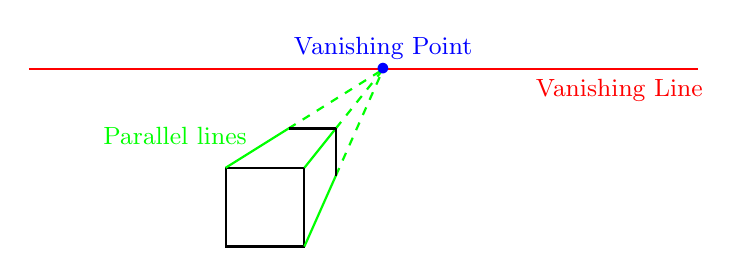
\begin{tikzpicture}[thick]
			\draw[] (0, 0) -- (1, 0) -- (1, 1) -- (0, 1) -- cycle;
			\draw[red] (-2.5, 2.25) -- (6, 2.25);
			\draw[green] (0, 1) -- (0.8, 1.5);
			\draw[green, dashed] (0.8, 1.5) -- (2, 2.25);
			\draw[green] (1, 1) -- (1.4, 1.5);
			\draw[green, dashed] (1.4, 1.5) -- (2, 2.25);
			\draw (0.8, 1.5) -- (1.4, 1.5);
			\draw[green] (1, 0) -- (1.4, 0.9);
			\draw[green, dashed] (1.4, 0.9) -- (2, 2.25);
			\draw (1.4, 0.9) -- (1.4, 1.5);
			
			\node[blue] (VP) at (2, 2.25) {$\bullet$};
			\node[above, blue] at (2, 2.25) {\small Vanishing Point};
			\node[below, red] at (5, 2.25) {\small Vanishing Line};
			\node[left, green] at (0.4, 1.4) {\small Parallel lines};
		\end{tikzpicture}
	\end{figure}

	\subsection{Special case of a tiled floor}
	
	This subsection will be useful for the last section of this report. There are two interesting equations to record about tiled floors linking tile lines with their diagonals. Indeed I will try to build a new painting that perfectly respects the perspective. But to do this, it is necessary to know the properties that the vanishing points of a tiled floor must respect.
	
	\begin{figure}[h]
		\centering
		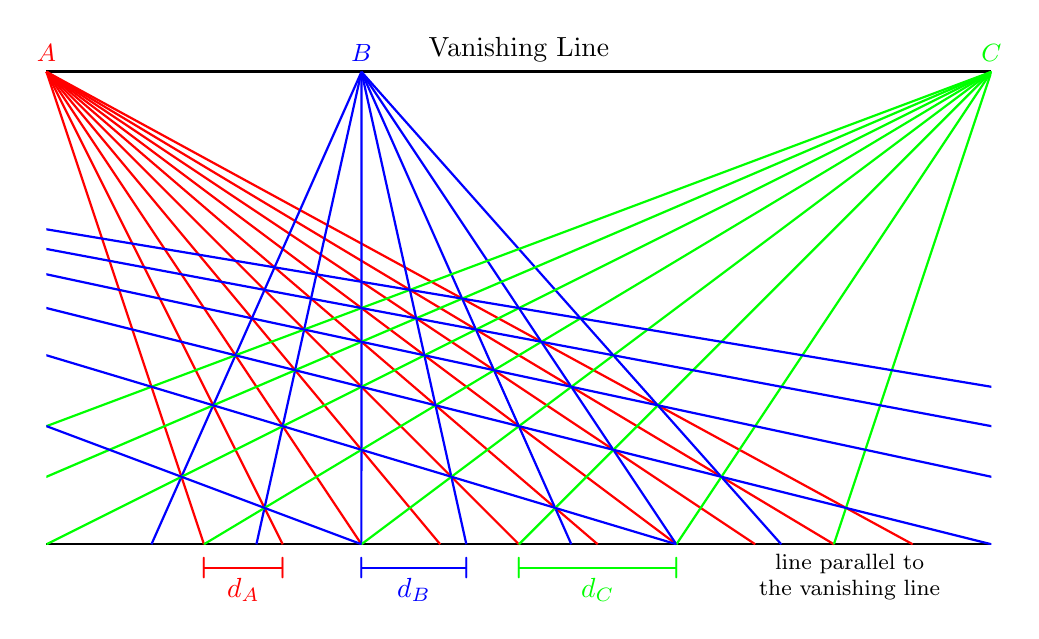
\begin{tikzpicture}[thick]
		\draw[very thick] (0, 6) -- (12, 6);
		\draw[semithick] (0, 0) -- (12, 0);
		\node[above] at (6, 6) {Vanishing Line};
		\node[above, red] at (0, 6) {\small $A$};
		\node[above, blue] at (4, 6) {\small $B$};
		\node[above, green] at (12, 6) {\small $C$};
		
		\foreach \i in {2, ..., 11} \draw[red] (0, 6) -- (\i, 0);
		\foreach \i in {1.333, 2.666, ..., 9.333} \draw[blue] (4, 6) -- (\i, 0);
		
		\draw[red] (2, -0.3) node {\texttt{|}} -- node[below] {$d_A$} (3, -0.3) node {\texttt{|}};
		\draw[blue] (4, -0.3) node {\texttt{|}} -- node[below] {$d_B$} (5.333, -0.3) node {\texttt{|}};
		\draw[green] (6, -0.3) node {\texttt{|}} -- node[below] {$d_C$} (8, -0.3) node {\texttt{|}};
		
		\node[below, align=center] at (10.2, 0)
			{\footnotesize line parallel to \\[-1mm]
			\footnotesize the vanishing line};
		
		\clip (0, 0) rectangle (12, 6);
		\foreach \i in {-4, -2, ..., 10} \draw[green] (12, 6) -- (\i, 0);
		\foreach \i in {4, 8, ..., 24} \draw[blue] (-12, 6) -- (\i, 0);
		\end{tikzpicture}
		\vspace{-2mm}
		\caption{Tiled floor in perspective}
		\label{im:tiledfloor}
	\end{figure}

	In the \figurename \ref{im:tiledfloor}, blue lines represent a tiled floor in perspective. We will always assume that tiles are squares. Then all the parallel lines are equally spaced. In perspective, this implies that if a line parallel to the vanishing line is drawn, then the tile lines intersect with it at regular intervals. We write these intervals $\color{blue} d_B$ for the depth lines, and $\color{red} d_A$ and $\color{green} d_C$ for the diagonals. $\color{red} A$, $\color{blue} B$ and $\color{green} C$ are the vanishing points located on the vanishing line (note that here the vanishing line is horizontal but it may not be). Finally here are the two equations respected by such a tiled floor:
	
	\begin{center}
		\begin{minipage}{0.3\linewidth}
			\begin{equation}
			{\color{blue} B} = \dfrac{{\color{green} d_C} {\color{red} A} + {\color{red} d_A} {\color{green} C}}{{\color{red} d_A} + {\color{green} d_C}}
			\end{equation}
		\end{minipage}
		\begin{minipage}{0.3\linewidth}
			\begin{equation}
			{\color{blue} d_B} = 2 \dfrac{{\color{red} d_A} {\color{green} d_C}}{{\color{red} d_A} + {\color{green} d_C}}
			\end{equation}
		\end{minipage}
	\end{center}
	
	\section{Description of the algorithm}
	
	% Need to talk about what I tried before hough transform (PCA on connex components)

	\subsection{General description}
	
	\subsection{Smoothing}
	
	\subsection{Gradient}
	
	\subsection{Hough Transform}
	
	\begin{figure}[h]
		\centering
		
\includegraphics[scale=1.2]{hough_painting.png}
		\caption{Hough Transform}
	\end{figure}

	\section{Attempt to redraw the paintings with a perfect perspective}

	\section{Conclusion}
	
	As a conclusion I did nothing during this internship !
	
	\appendix
	
	\section{Source Code}
	
	Here is my git repository: \url{https://github.com/Nanored4498/Painting-Analysis}.

	\bibliographystyle{alpha}
	\bibliography{bib.bib}
	
\end{document}